\documentclass[serif,xcolor=pdftex,dvipsnames,table,hyperref={bookmarks=false,breaklinks}]{beamer}

%%%%%%%%%%%%%%%%
% Change the macros below to configure the title slides
% for your course.
\newcommand{\coursename}{COMPSCI 590N}
\newcommand{\instructor}{Roy J. Adams}
\newcommand{\university}{University of Massachusetts Amherst}
\newcommand{\department}{College of Information and Computer Sciences}
%%%%%%%%%%%%%%%%

\newcommand\HUGE{\@setfontsize\Huge{50}{60}}

\newcommand{\settitlecard}[2]{
  \title[\coursename  Lecture #1] 
    {\coursename \\ Lecture #1: #2}
     \author[\instructor]{\instructor}
     \institute[\university]{
     \department\\
     \university
   }
\date{}
}

\newcommand{\maketitlepage}{
  \begin{frame}
  \titlepage
  %\center{
    %If you use the slides unmodified, retain the attribution below
  %  \tiny{Slides by Roy J. Adams (rjadams@cs.umass.edu). 
    %If you modify the slides, please retain the alternate attribution below
    %\tiny{Based on slides by Roy J. Adams (rjadams@cs.umass.edu). \\    
  %  }                                              
  %}  
  \end{frame}
}

\AtBeginSection[]
{
  \begin{frame}<beamer>{Outline}
    \tableofcontents[currentsection,subsectionstyle=hide]
  \end{frame}
}


\newcommand{\cut}[1]{}

\newcommand{\iconbox}[4]{
  \only<#1-#2>{
    \begin{columns}[T]
      \column{0.5in}
           \includegraphics[width=0.5in]{#3}
       \column{3.7in}
            #4
    \end{columns}
    \medskip
    \medskip
    \medskip
  }
}

\mode<presentation>{
  \usepackage{../beamertheme589theme}
  \setbeamercovered{invisible}
}

\mode<handout>{
  \usepackage{../beamertheme589theme}
  \setbeamercovered{transparent}
}


\usepackage[english]{babel}
\usepackage[latin1]{inputenc}
\usepackage{times}
\usepackage[T1]{fontenc}
\usepackage{amsmath}
\usepackage{amssymb}
\usepackage[noend]{algorithmic}
\usepackage{algorithm}
\usepackage{listings}
\usepackage{tcolorbox}
\usepackage{xmpmulti}

\renewcommand\mathfamilydefault{\rmdefault}

\newcommand{\setA}{\mathcal{A}}
\newcommand{\setB}{\mathcal{B}}
\newcommand{\setS}{\mathcal{S}}
\newcommand{\setV}{\mathcal{V}}
\DeclareMathOperator*{\union}{\bigcup}
\DeclareMathOperator*{\intersection}{\bigcap}
\DeclareMathOperator*{\Val}{Val}
\newcommand{\mbf}[1]{{\mathbf{#1}}}
\DeclareMathOperator*{\argmax}{arg\,max}
\DeclareMathOperator*{\argmin}{arg\,min}
\DeclareMathOperator*{\sign}{sign}
\newcommand{\deriv}[2]{\frac{\partial{#1}}{\partial{#2}}}

\lstdefinestyle{custompython}{
  belowcaptionskip=1\baselineskip,
  breaklines=true,
  frame=single,
  xleftmargin=\parindent,
  language=Python,
  showstringspaces=false,
  basicstyle=\footnotesize\ttfamily,
  keywordstyle=\bfseries\color{green!40!black},
  commentstyle=\itshape\color{purple!40!black},
  identifierstyle=\color{blue},
  stringstyle=\color{orange},
}
\lstset{style=custompython}

\makeatletter
\renewcommand*\env@matrix[1][*\c@MaxMatrixCols c]{%
  \hskip -\arraycolsep
  \let\@ifnextchar\new@ifnextchar
  \array{#1}}
\makeatother

\newcommand\norm[1]{\left\lVert#1\right\rVert}


\settitlecard{9}{Sparse Matrices and Probability 1}

\begin{document}

\maketitlepage

\section{Sparse Matrices}
\subsection{Foo}

\begin{frame}[t]{Sparsity}
	\begin{itemize}[<+->]
		\item A \textbf{sparse matrix} is an matrix in which most of the entries are zero. 
		\item This is in contrast to a \textbf{dense matrix}.
		\item Sparse matrices naturally appear in many applications:
		\begin{itemize}[<+->]
			\item Network adjacency matrices are typically very sparse. For example, you are only Facebook friends with a small percentage of the total Facebook population.
			\item In recommender systems, ratings are often arranged as a sparse matrix. 
			\item In NLP, the matrix of word counts in a set of documents is typically sparse.
			\item Multiple parallel event sequences can be arranged as a matrix. If the events are uncommon, then the matrix is sparse.
		\end{itemize}
		\item If we know an matrix is sparse, we can take advantage of this structure to speed up computations on the matrix.
	\end{itemize}
\end{frame}

\begin{frame}[t]{Sparsity}
	\begin{itemize}[<+->]
		\item Consider taking the inner product of two length $n$ vectors, $x$ and $y$.
		\item In general, how many multiplications must we perform?
		\item What if we know that only 10\% of the entries in $x$ are non-zero and we know where the are, how many multiplications do we need to perform?
	\end{itemize}
\end{frame}

\begin{frame}[t]{Sparse Representations}
	There are two main strategies for storing sparse matrices:
	\begin{enumerate}[<+->]
		\item Formats that support \textbf{efficient modifications} include Dictionary of Keys (DOK), List of Lists (LIL), and Coordinate list (COO) formats.
		\item Formats that support \textbf{efficient access and operations} include Compressed Sparse Row (CSR) and Compressed Sparse Column (CSC) formats.
	\end{enumerate}
\end{frame}

\begin{frame}[t]{Dictionary of Keys Format}
	\begin{itemize}[<+->]
		\item The DOK format is perhaps the simplest of the formats for efficient modification. 
		\item The DOK format stores the matrix as a dictionary with row/column tuples as keys and one key/value pair per non-zero entry.
		\item Adding or removing an entry can be done in constant time. 
		\item What is the complexity of row or column slicing?
	\end{itemize}
\end{frame}

\begin{frame}[t,fragile]{Compressed Sparse Row Format}
	\begin{itemize}[<+->]
		\item The CSR format stores an $m \times n$ matrix as three one dimensional arrays \verb|indices|, \verb|indptr|, and \verb|data|.
		\begin{enumerate}[<+->]
			\item The \verb|data| array stores the non-zero entries of the matrix in a left-to-right top-to-bottom order (row major order).
			\item The \verb|indices| array has the same length as the \verb|data| array and stores the column of each entry.
			\item The \verb|indptr| array is a length $m$ array. \verb|indptr[i]| stores the index in \verb|data| and \verb|indices| of the first non-zero entry in the $i$th row.
		\end{enumerate}
		\item The CSC format is the same as CSR, but \verb|data| is stored in column major order and \verb|indices| stores the row of each entry.
	\end{itemize}
	
\end{frame}

\begin{frame}[t]{Compressed Sparse Row Format: Example}
	\centering
	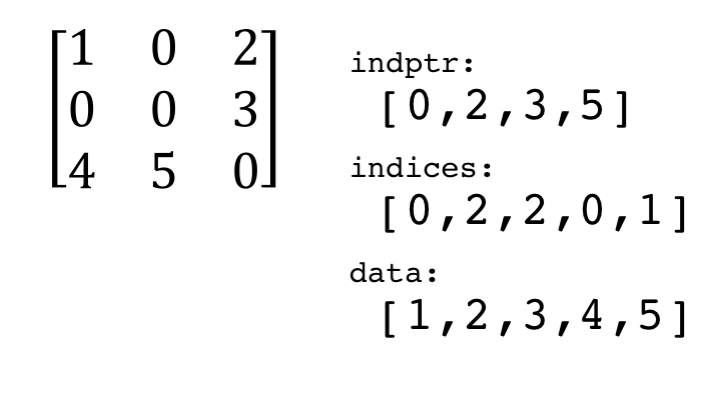
\includegraphics[width=\textwidth]{{../Figures/array_slicing/Slide32}.png}
\end{frame}

\begin{frame}[t]{Compressed Sparse Row Format: Example}
	\centering
	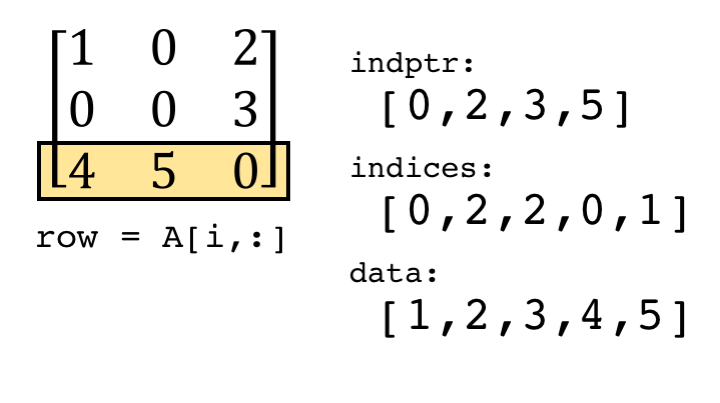
\includegraphics[width=\textwidth]{{../Figures/array_slicing/Slide33}.png}
\end{frame}

\begin{frame}[t]{Compressed Sparse Row Format: Example}
	\centering
	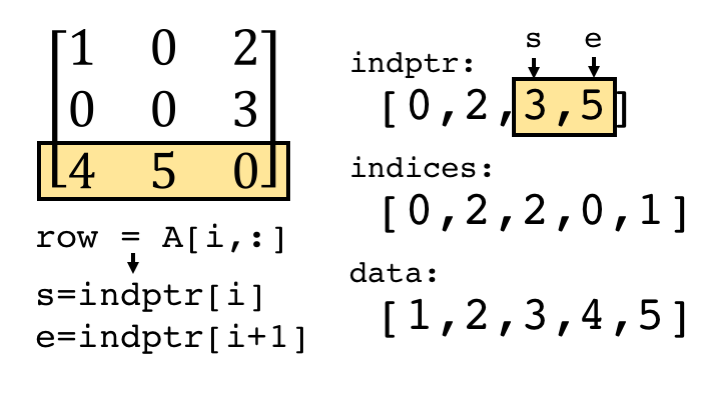
\includegraphics[width=\textwidth]{{../Figures/array_slicing/Slide34}.png}
\end{frame}

\begin{frame}[t]{Compressed Sparse Row Format: Example}
	\centering
	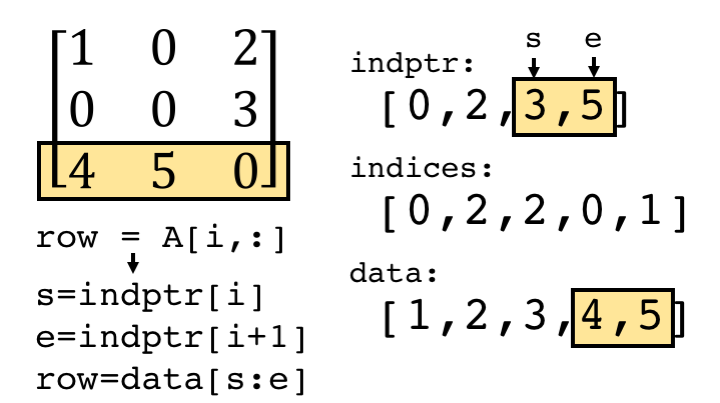
\includegraphics[width=\textwidth]{{../Figures/array_slicing/Slide35}.png}
\end{frame}

\begin{frame}[t]{Compressed Sparse Row Format: Example}
	\centering
	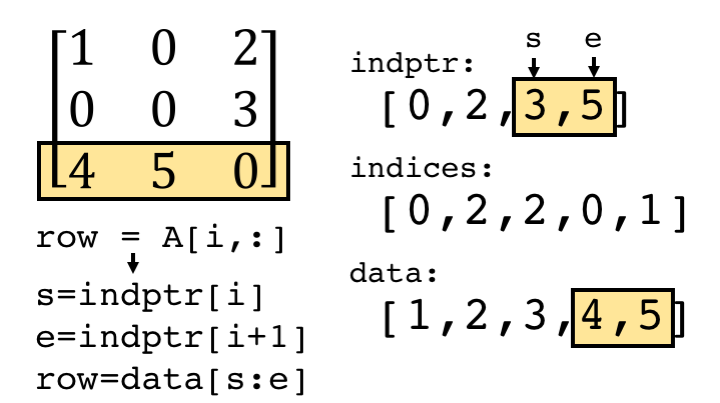
\includegraphics[width=\textwidth]{{../Figures/array_slicing/Slide35}.png}
\end{frame}

\begin{frame}[t,fragile]{Scipy Sparse Matrices}
	The module \verb|scipy.sparse| implements each of these sparse formats.
	
	\begin{lstlisting}
		>>> import scipy.sparse as sps
		>>> import numpy as np
		
		>>> A = np.eye(5)
		>>> identity = np.eye(5)
		>>> sparse_identity = sps.csr_matrix(identity)
		
		>>> sparse_identity.indptr
		array([0, 1, 2, 3, 4, 5], dtype=int32)
		>>> sparse_identity.indices
		array([0, 1, 2, 3, 4], dtype=int32)
		>>> sparse_identity.data
		array([ 1.,  1.,  1.,  1.,  1.])
	\end{lstlisting}
\end{frame}

\begin{frame}[t,fragile]{Interactive Demo}
	\begin{itemize}
		\item What linear algebra operations are most sped up by using sparse matrices?
	\end{itemize}
\end{frame}

\section{Probability in Python}
\subsection{Foo}

\begin{frame}[t]{Random Variables}
	% PDF, PMF, CDF
	\begin{itemize}[<+->]
		\item Probability and statistics play a central role in data analysis, modeling, and numerical algorithms. 
		\item But first, a quick review.
	\end{itemize}
	
	\pause
	\begin{block}{Random Variables}
		A random variable, $X$, is a quantity that can take any value from a set of possible values, $\Omega$, according to a set of probabilities.
	\end{block}
\end{frame}
	
\begin{frame}[t]{Random Variables}
	For example: Imagine we are flipping a coin. 
	\pause
	\begin{itemize}[<+->]
		\item What is the random variable?
		\begin{itemize}[<+->]
			\item The random variable is the outcome of the coin flip.
		\end{itemize}
		\item What is the set of possible outcomes?
		\begin{itemize}[<+->]
			\item $\Omega = \{H,T\}$
		\end{itemize}
	\end{itemize}
	
\end{frame}

\begin{frame}[t]{Discrete Random Variables}
	% PDF, PMF, CDF
	\begin{itemize}[<+->]
		\item A discrete random variable may take its value from a finite or countably infinite set.
		\item Examples include:
		% Support as a question
		\begin{itemize}[<+->]
			\item The outcome of a coin flip can take one of two possible values.
			\item A randomly dealt five card poker hand can take one of $\approx$2.6 possible million values.
			\item The number of people who log in to Netflix between 1pm and 2pm can be any non-negative integer.
			\item The end of season goal differential for a soccer team can be any integer (positive or negative).
		\end{itemize}
	\end{itemize}
\end{frame}

\begin{frame}[t]{Probability Mass Functions}
	% PDF, PMF, CDF
	The probability of each possible outcome is defined by a Probability Mass Function.
	
	\begin{block}{Probability Mass Function}
		For a discrete random variable $X$ with support $\Omega$, a Probability Mass Function (PMF) $P:\Omega\to [0,1]$ maps possible outcomes to probabilities. A PMF must satisfy two conditions:
		\begin{enumerate}[<+->]
			\item Probability of any single outcome must be between zero and one (i.e. $P(x) \in [0,1]$ for all $x \in \Omega$).
			\item The probabilities of all possible outcomes must sum to one (i.e. $\sum_x P(x) = 1$).
		\end{enumerate}
	\end{block}
\end{frame}

\begin{frame}[t]{Probability Mass Functions: Examples}
	% PDF, PMF, CDF
	Let $X$ represent the outcome of a six sided dice roll.
	\begin{itemize}[<+->]
		\item The set of possible outcomes is $\Omega = \{1,2,3,4,5,6\}$.
		\item Assuming the dice is fair, then the PMF may look like:
	\end{itemize}
	\pause
	% Dice PMF
	\centering
	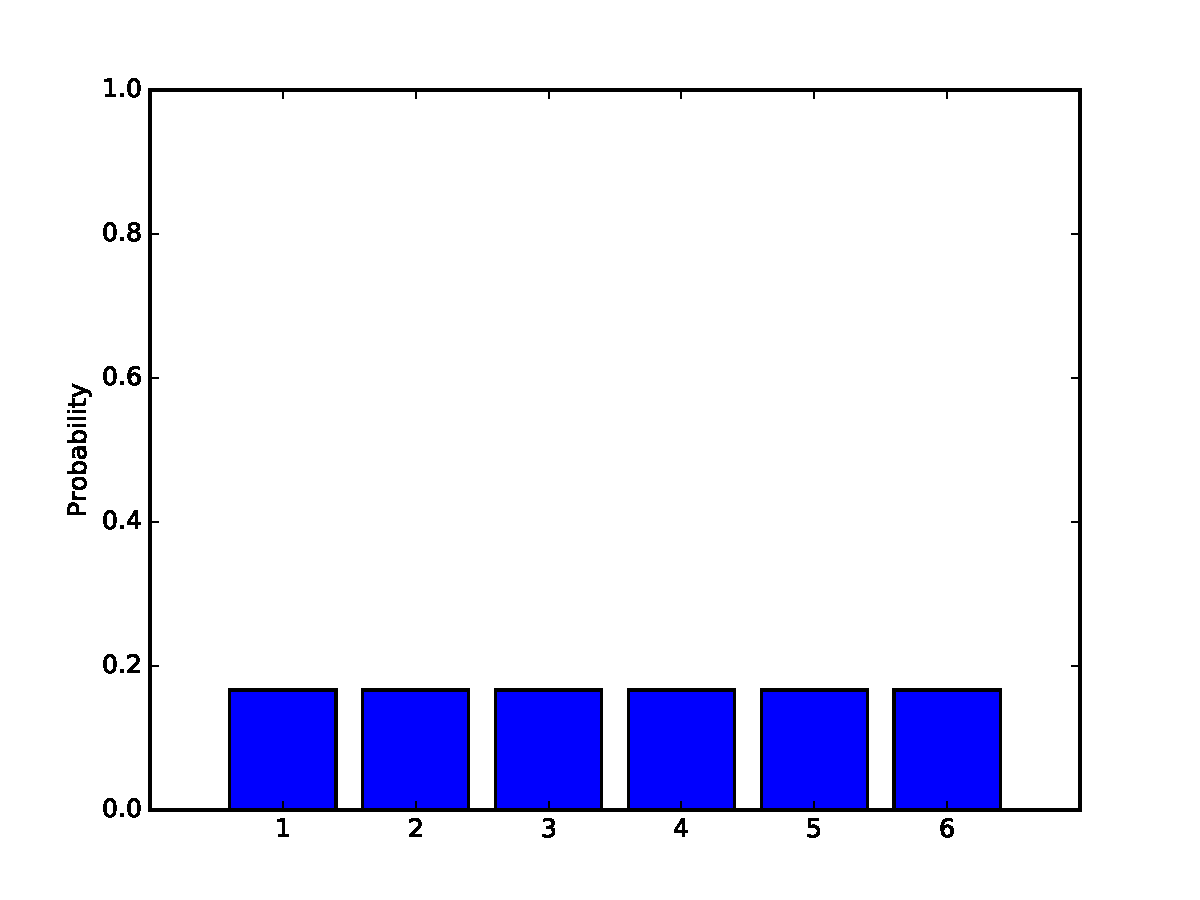
\includegraphics[height=2in]{../Figures/uniform_multinomial.pdf}
\end{frame}

\begin{frame}[t]{Probability Mass Functions: Examples}
	% PDF, PMF, CDF
	Let $X$ represent the the number of people entering a certain bank between 1pm and 2pm.
	\begin{itemize}[<+->]
		\item The set of possible outcomes is the set of all non-negative integers $\Omega = \mathbb{Z}_{\geq 0}$.
		\item This random variable is a canonical example of a Poisson distributed random variable which has the following PMF:
	\end{itemize}
	\pause
	% Poisson PfMF
	\centering
	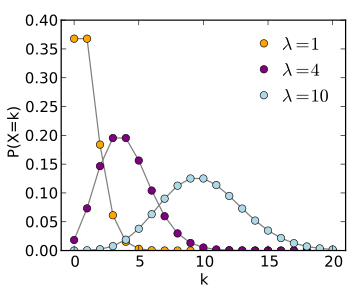
\includegraphics[height=1.5in]{../Figures/Poisson_pmf.png}
\end{frame}

\begin{frame}[t]{Parametric Distributions}
	The Poisson distribution is an example of a \textbf{parametric distribution}, that is, it requires a set of parameter values to fully specify the distribution.
	
	\pause
	\begin{align*}
		f(X=x; \lambda) = \frac{\lambda^x e^{-\lambda}}{x!},\, \lambda > 0
	\end{align*}
	
	\pause
	\begin{itemize}[<+->]
		\item In this case the, the distribution has a single parameter $\lambda$ that must be a positive real number. 
		\item Much of statistics is concerned with inferring these parameters from data.
	\end{itemize}
\end{frame}

\begin{frame}[t]{Continuous Random Variables}
	\begin{itemize}[<+->]
		\item A continuous random variable takes its value from an uncountably infinite set such as the set of real numbers. 
		\item Examples include:
		\begin{itemize}[<+->]
			\item The height of a randomly selected person.
			\item Income of a randomly selected household.
			\item The amount of time between hard drive failures in a server.
		\end{itemize}
	\end{itemize}
\end{frame}

\begin{frame}[t]{Probability Density Functions}
	The distribution over possible values of a continuous random variable is given by a \textbf{probability density function}.
	\begin{block}{Probability Density Function}
		For a continuous random variable $X$, the probability density function (PDF) $P(x)$ describes the relative likelihood of a continuous random variable taking a given value. A PDF must satisfy the following two conditions:
		\begin{enumerate}[<+->]
			\item All values must be non-negative. That is, $P(x) \geq 0$ for all $x \in \Omega$.
			\item The area under the PDF must equal one. That is, $\int_x P(x) dx = 1$.
		\end{enumerate}
		\pause
		The probability of $X$ falling between $a$ and $b$ is given by the integral:
		$$P(a < x < b) = \int_x p(x) dx$$
	\end{block}
\end{frame}

\begin{frame}[t]{Probability Density Functions: Examples}
	\begin{itemize}
		\item Given some range $[a,b]$, the \textbf{uniform distribution} places equal likelihood on all values in the range.
	\end{itemize}
	\pause
	\begin{align*}
		p(x;a,b) = \frac{1}{b - a}
	\end{align*}
	% uniform plot
	\centering
	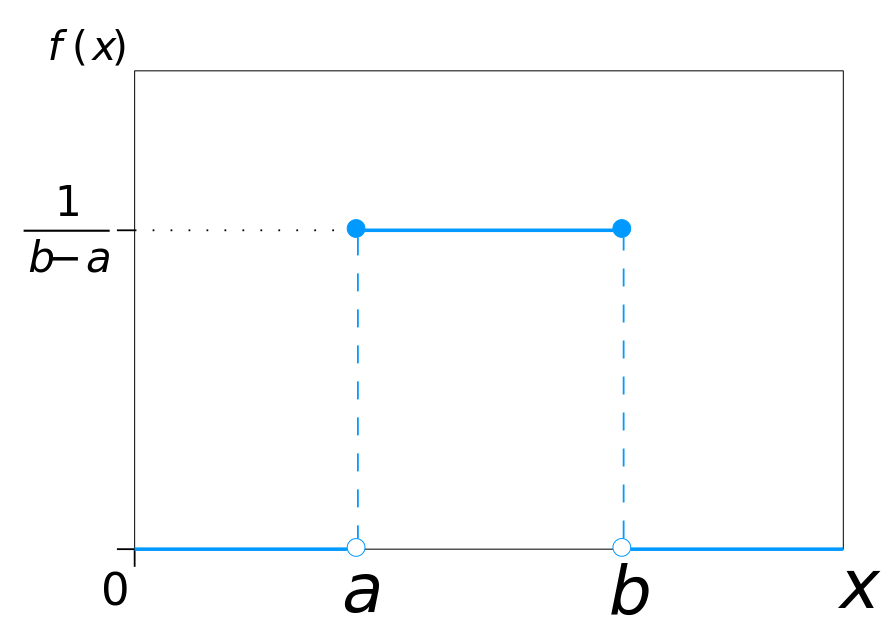
\includegraphics[height=1.5in]{../Figures/Uniform_Distribution_PDF_SVG.png}
\end{frame}

\begin{frame}[t]{Probability Density Functions: Examples}
	\begin{itemize}[<+->]
		\item Perhaps the most common distribution in statistics is the \textbf{Normal} distribution.
		\item The Normal distribution takes two parameters: a mean parameter $\mu$ and a variance parameter $\sigma^2$.
	\end{itemize}
	\pause
	\begin{align*}
		p(x;\mu,\sigma) = \frac{1}{\sqrt{2\pi\sigma^2}}\exp\left(-\frac{(x-\mu)^2}{2\sigma^2}\right)
	\end{align*}
	% Normal plot
	\centering
	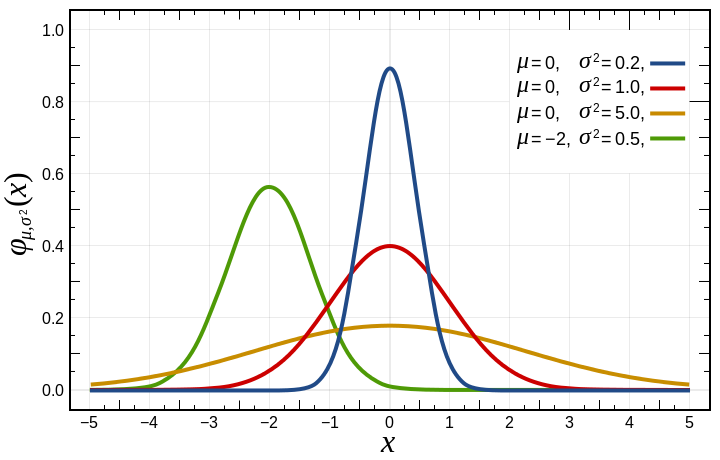
\includegraphics[height=1.5in]{../Figures/Normal_Distribution_PDF.png}
\end{frame}

% \begin{frame}[t]{Cumulative Mass Function}
% 	\begin{block}{Cumulative Mass Function}
% 		A Cumulative Mass Function (CMF) is
% 	\end{block}
% \end{frame}

\begin{frame}[t]{Evaluating PMFs, PDFs, and CMFs}
	The most fundamental computation necessary when working with probability distributions is evaluating the distribution at different values. This computation can be difficult or costly for a number of reasons:
	\pause
	\begin{itemize}[<+->]
		\item The PDF, PMF, or CMF involves a difficult to compute special function.
		\item Normalizing the distribution (ensuring the PDF/PMF integrates to 1) requires a difficult to compute sum or integral.
		\item Probabilities near zero or near one can cause numerical errors.
	\end{itemize}
\end{frame}

\begin{frame}[t]{Calculating PDFs: The Gamma Function}
	Evaluating PDFs and PMFs, even common ones, often requires evaluating difficult to compute special functions. A particularly common function for continuous distributions is the Gamma function.

	\pause
	\begin{block}{Gamma Function}
		The gamma function is defined as
		$$\Gamma(t) = \int_0^\infty x^{t-1}e^{-x}dx$$
	\end{block}

	\pause
	The Gamma function and related Incomplete Gamma and Incomplete Beta functions are necessary/useful for working with the following common distributions (among others).
	\begin{itemize}[<+->]
		\item Gamma, $Z$, $t$, $\chi^2$, $F$, binomial, Poisson
	\end{itemize}
\end{frame}

\begin{frame}[t]{Calculating PDFs: The Gamma Function}
	Algorithms for computing the Gamma function have been heavily studied. The most commonly used algorithm is uses the Lanczos approximation.

	\pause
	\begin{align*}
		\Gamma(z+1) &= \sqrt{2\pi}\left(z + g + \frac{1}{2}\right)^{z+1/2}e^{-(z+g+1/2)}A_g(z)\\
		A_g(z) &= c_0 + \frac{c_1}{z+1} + \frac{c_2}{z+2} + \frac{c_3}{z+3} + ... \\
	\end{align*}

	\pause
	Importantly, the user can choose $g$ and pre-calculate the constants $c_i$.
\end{frame}

\begin{frame}[t]{Calculating PMFs: Using Recursion}
	\begin{itemize}[<+->]
		\item Often, when multiple values of a PMF are desired, we can take advantage of recurrence relations to avoid calculating costly special functions.
		\item The binomial distribution is the distribution for the number of successes in a sequence of $n$ yes/no experiments (e.g. coin flips) with success probability $p$. The binomial PMF is,
	\end{itemize}
	\pause
	\begin{align*}
		P(X = x; n, p) &= {{n}\choose{x}}p^x(1-p)^{n-x}
	\end{align*}
\end{frame}

\begin{frame}[t]{Calculating PMFs: Using Recursion}
	Evaluating the binomial PMF involves evaluating factorials (a special case of the Gamma function); however, if multiple values are desired, we can take advantage of the following recurrence relation:

	\begin{align*}
		P(X=x) &= {{n}\choose{x}}p^x(1-p)^{n-x}\\
		&= \frac{n-x}{x+1}\frac{p}{1-p}\left[{{n}\choose{x-1}}p^{x-1}(1-p)^{n-(x-1)}\right]\\
		&= P(X=x-1)\frac{n-x}{x+1}\frac{p}{1-p}
	\end{align*}
\end{frame}

\begin{frame}[t]{Calculating PMFs: Using Recursion}
	\begin{itemize}[<+->]
		\item Does utilizing this recursion improve the complexity or the constant?
		\item The complexity of calculating the first $k$ values of the binomial PMF is $\mathcal{O}(k)$ in both cases; however, we are replacing a special function with arithmetic operations only.
	\end{itemize}
\end{frame}

\begin{frame}[t]{Working in log-space and the Log-Sum-Exp trick}
	\begin{itemize}[<+->]
		\item As we discussed in a previous lecture, exponentiating even moderate values can result in numerical overflow or underflow.
		\item Many distributions require exponentiation of intermediate values.
		\item One common solution is to work in \textbf{log-space}.
	\end{itemize}
	
\end{frame}


\begin{frame}[t]{Working in log-space and the Log-Sum-Exp trick}
	The multinomial distribution is the standard distribution for finite sets. Consider the following multinomial distribution over $K$ discrete values parameterized by a length $K$ vector of weights $\alpha$.
	
	\begin{align*}
		P(X=i; \alpha) &= \frac{e^{\alpha_i}}{\sum_i e^{\alpha_i}},\, i = 1,...,K
	\end{align*}
	
	\pause
	Rather than evaluate this function directly, risking over/underflow, we can evaluate the log PMF,
	
	$$\log P(X=i;\alpha) = \alpha_i - \log \sum_i e^{\alpha_i}$$
	
	\pause
	Why does this not completely solve our problem?
	
\end{frame}

\begin{frame}[t]{Working in log-space and the Log-Sum-Exp trick}
	Calculating the second term $\log \sum_i e^{\alpha_i}$ (also known as the cumulant function) still requires exponentiating $\alpha$. Instead, let $\alpha^* = \max_i \alpha_i$. Then, we can use the following trick,
	
	\begin{align*}
		\log \sum_i e^{\alpha_i} &= \log \frac{e^{\alpha^*}}{e^{\alpha^*}}\sum_i e^{\alpha_i}\\
		&= \log \sum_i e^{\alpha_i-\alpha^*} + \log e^{\alpha^*}\\
		&= \log \sum_i e^{\alpha_i-\alpha^*} + \alpha^*\\
	\end{align*}
\end{frame}
	
\begin{frame}[t,fragile]{Working in log-space and the Log-Sum-Exp trick}
	\begin{itemize}[<+->]
		\item Now we are guaranteed that the largest term in the sum equals one.
		\item There can be no overflow and, while individual terms in the sum may underflow, this results only in round-off error in the final sum.
		\item Log-sum-exp is implemented in \verb|scipy.misc.logsumexp|.
	\end{itemize}
\end{frame}

% \begin{frame}[t]{Estimating and Visualizing Distributions}
% 	% PDF, PMF, CDF
% \end{frame}
%
% \begin{frame}[t]{Building Histograms}
% 	% PDF, PMF, CDF
% \end{frame}
%
% \begin{frame}[t]{Seaborn}
% \end{frame}
%
% \begin{frame}[t]{Seaborn}
% 	% Interactive Demo
% \end{frame}

\end{document}
